\documentclass[conference]{IEEEtran}
\IEEEoverridecommandlockouts

\usepackage{cite}
\usepackage{amsmath,amssymb,amsfonts}
\usepackage{graphicx}
\usepackage{booktabs}
\usepackage{textcomp}
\usepackage{xcolor}
\usepackage{tikz}
\usetikzlibrary{arrows.meta,positioning,fit,calc}
\usepackage[hidelinks]{hyperref}

% Draft-visible placeholder for metrics pending the training rerun
\newcommand{\phX}{{\color{red}[X]}}

\begin{document}

\title{Beyond Human Vigilance: A CCTV-Based Deep Learning System for Real-Time PPE Compliance Detection in Industrial Sites}

\author{
\IEEEauthorblockN{Amine Zeguendry}
\IEEEauthorblockA{\textit{Cadi Ayyad University}\\
\textit{LAMIGEP Research Laboratory, EMSI}\\
Marrakech, Morocco}
\and
\IEEEauthorblockN{Yasser Dalali}
\IEEEauthorblockA{\textit{LAMIGEP Research Laboratory, EMSI}\\
Marrakech, Morocco\\
yasser.dalali@emsi-edu.ma}
\and
\IEEEauthorblockN{Mohammed Taha Eladli}
\IEEEauthorblockA{\textit{LAMIGEP Research Laboratory, EMSI}\\
Marrakech, Morocco\\
taha.eladi@emsi-edu.ma}
}

\maketitle

\begin{abstract}
% Abstract body only — \input inside the abstract environment in main.tex.
Work-related accidents kill nearly three million people each year and cost an estimated 4\% of global GDP, yet the IP camera networks already installed across industrial sites still depend on human observers whose sustained attention collapses within 20--35 minutes. Automated PPE detection could close that gap, but published systems are trained and evaluated on construction-centric benchmarks and, to our knowledge, none has been evaluated on imagery from a real, operating chemical plant. This paper presents a PPE compliance pipeline developed for and evaluated at OCP Group phosphate-processing facilities (specifically at Safi's Maroc Chimie chemical plant). A YOLOv8n detector (3.0M parameters) is fine-tuned at $640\times640$ resolution on a composite industrial dataset (the public Roboflow PPE-Detection corpus, SH17 dataset (capped), the Roboflow gas masks corpus, and weighted site-specific OCP imagery) that covers the gas masks, IP camera viewing angles, and site uniforms construction benchmarks omit. The central experiment compares this industrial-adapted model against a detector trained only on the standard construction benchmark: on held-out chemical-plant imagery the adapted model reaches 65.5\% mAP@50 against 18.5\% for the generic baseline, with a wider gap still on an industrial proxy test set (49.6\% against 0.4\%). The gap is evidence that generic benchmark training does not transfer to operating-plant conditions, and that the contribution is domain-specific rather than architectural. The pipeline requires no new camera hardware and retrofits onto the IP camera infrastructure a site already operates.

\end{abstract}

\begin{IEEEkeywords}
PPE compliance, YOLOv8, vigilance decrement, LLM-based alert verification, industrial safety, computer vision, CCTV retrofitting
\end{IEEEkeywords}

\section{Introduction}\label{sec:intro}

Work-related accidents and diseases kill nearly three million people every year, 395 million workers sustain non-fatal injuries \cite{ilo2023}, and the economic burden approaches 4\% of global GDP \cite{ilo2023,lloyds2024}; in the United States alone it reached \$176.5 billion in 2023 \cite{nsc2023}. In heavy industry, personal protective equipment (PPE) is often the last barrier between a hazard and a worker, but a PPE mandate is only as effective as its enforcement. On most industrial sites, enforcement still means a human operator watching a wall of CCTV monitors.

That arrangement fails for a well-documented reason: vigilance is a rapidly depleting resource. Laboratory studies show detection performance collapsing within 20--35 minutes of continuous monitoring \cite{parasuraman1984,sawin1995}; surveillance-literature estimates suggest operators miss up to 95\% of on-screen activity after 22 minutes \cite{velastin2006}; and trained operators watching live feeds in diamond-processing plants detected only about half of targeted risk behaviors while generating high false-alarm rates \cite{donald2015}, with attention lapses accumulating over 90-minute sessions \cite{sandia2014}. A single camera produces 525{,}600 minutes of footage per year and an accident occupies roughly one of them. Manual surveillance pays off only if the operator is fully attentive during that exact minute.

Automated PPE detection promises to remove this bottleneck, and YOLO-family detectors dominate the field \cite{ultralytics2023,ppeyolo2024,edgeyolo2024}. Yet published systems are built and evaluated on construction-centric, lab-clean benchmarks; to our knowledge, none has been evaluated on imagery from a real, operating chemical plant. Two gaps produce that vacuum. First, the training data: public benchmarks such as Roboflow PPE-Detection \cite{roboflowppe} and the 17-class SH17 \cite{ahmad2024sh17} revolve around helmets and high-visibility vests and under-represent both the classes chemical operations depend on (gas masks, goggles) and the conditions of a phosphate-processing site (dust, harsh lighting, uniforms that generic models mistake for PPE). Second, few systems adapt to an individual site at all, even though that domain shift is precisely where generic detectors break down. This paper's central experiment measures the breakdown directly.

This paper addresses these gaps with a CCTV-retrofit PPE compliance system developed for, and evaluated at, OCP Group in Morocco. Its core claim is domain-specific rather than architectural: a detector fused and adapted for industrial and chemical conditions (oblique CCTV viewing angles, gas masks, site-specific uniforms) outperforms a detector trained only on the standard construction benchmark when both face chemical-plant imagery. Our contributions are:
\begin{itemize}
  \item \textbf{Real-plant central experiment.} A controlled comparison between a generic detector trained solely on the public construction benchmark \cite{roboflowppe} and our industrial-adapted model, on held-out OCP chemical-plant imagery and an industrial proxy set. The comparison, not a new architecture, is the claim.
  \item \textbf{Composite domain-adapted dataset.} A fusion of Roboflow PPE-Detection \cite{roboflowppe}, SH17 \cite{ahmad2024sh17}, the Roboflow gas masks corpus \cite{roboflowgasmasks}, and a self-annotated OCP corpus with weighted site-specific sampling, the dataset whose effect the central experiment measures.
  \item \textbf{Retrofit deployment model.} The pipeline runs on existing camera and network infrastructure; alerts reach the channels safety staff already use.
\end{itemize}

Section~\ref{sec:related} reviews related work; Section~\ref{sec:methods} details the dataset, comparison protocol, and system; Section~\ref{sec:results} presents results; Sections~\ref{sec:discussion} and~\ref{sec:conclusion} discuss limitations and conclude.

\section{Related Work}\label{sec:related}

Automated PPE detection has consolidated around the YOLO family of one-stage detectors, whose inference speed makes them the default choice for video-rate safety applications \cite{ultralytics2023}. Recent YOLOv8-based studies benchmark helmet and vest detection across public object-detection datasets \cite{ppeyolo2024}, and edge-deployed variants extend the approach to preventing falls from height on construction sites, confirming that real-time PPE monitoring is feasible on modest hardware \cite{edgeyolo2024}. Community resources such as the Roboflow Universe PPE-Detection corpus \cite{roboflowppe} supply most of the training data behind this line of work and have made baseline detectors straightforward to reproduce. The shared limitation is scope. These benchmarks are construction-centric: their class inventories revolve around hard hats and high-visibility vests, while the respiratory and eye protection that dominates compliance requirements in chemical processing---gas masks, goggles---is absent. None of them adapts the detector to the visual conditions of a specific site, where dust, harsh lighting, and uniforms that resemble PPE degrade models trained on clean public imagery.

The SH17 dataset \cite{ahmad2024sh17} broadens the label space to seventeen classes spanning PPE items and human body parts in manufacturing scenes, currently the widest public inventory for industrial PPE detection. Its breadth, however, is deliberately generic: the imagery reflects general manufacturing rather than chemical-industry environments, and the dataset carries no mechanism for the domain shift a detector encounters when moved onto a particular plant's cameras. SH17 is a strong ingredient for a site-adapted model, not a substitute for one.

A separate literature explains why automated detection is needed at all. Classical sustained-attention research established that vigilance decays within the first half hour of a continuous monitoring task \cite{parasuraman1984}, and that the decrement persists even when observers are explicitly instructed and motivated \cite{sawin1995}. CCTV-specific evidence points the same way. Velastin et al. proposed motion-based video analysis for underground stations on the premise that human operators cannot reliably watch large banks of monitors \cite{velastin2006}, and a Sandia National Laboratories assessment of continuous monitoring tasks describes attention lapses that spread across operators as sessions extend \cite{sandia2014}. The most direct evidence for industrial CCTV comes from Donald, Donald, and Thatcher, who studied trained surveillance operators in diamond-processing plants and reported that they detected roughly half of the targeted risk behaviours while generating a high rate of false alarms \cite{donald2015}. That second finding matters as much as the first. A detector that merely replaces the human eye trades missed events for a stream of false alerts, shifting the vigilance burden downstream to whoever triages the alarms rather than removing it. The false-alarm half of that result is the specific failure mode our verification stage is built against: no alert should reach safety staff before a reasoning pass has examined why the detection might be wrong.

Vision-language models are a natural candidate for that verification role. Recent reviews chart rapid progress in VLMs for object detection and segmentation \cite{vlmreview2025}, and open-weight models such as Qwen2.5-VL bring grounded visual reasoning to hardware that an industrial operator can run on premises \cite{qwen25vl}. Detect-then-reason pipelines, in which a fast detector proposes candidate events and a slower model judges them with scene context, follow directly from these capabilities. Yet the pattern remains nascent, and applications to safety monitoring---where occlusion, glare, and distance routinely produce the kind of ambiguous detection that contextual reasoning could resolve---are rare.

Each thread therefore stops short of our setting. Detection research offers fast, reproducible models but only generic, construction-centric classes and no site adaptation; SH17 widens the label space without reaching chemical-industry classes or conditions; the vigilance literature diagnoses manual monitoring as structurally unreliable and warns that false alarms recreate the problem downstream, but offers no detection-side remedy; and VLM-based verification exists in principle but not in deployed safety pipelines. No prior work, to our knowledge, joins site-adapted detection over chemical-industry PPE classes with a reasoning-based false-positive filter on retrofit CCTV infrastructure. Table~\ref{tab:relwork} summarizes the closest prior efforts and what each contributes to that combined gap.

\begin{table}[t]
\caption{Summary of Related Work Across the Three Threads}
\label{tab:relwork}
\centering
\footnotesize
\setlength{\tabcolsep}{3pt}
\begin{tabular}{p{1.9cm}p{1.6cm}p{1.9cm}p{2.5cm}}
\toprule
\textbf{Study/Source} & \textbf{Method} & \textbf{Focus} & \textbf{Key Finding} \\
\midrule
Roboflow PPE-Detection \cite{roboflowppe} & Public YOLO-format dataset & Helmet/vest detection & Widely reused baseline; construction-centric class set \\
\addlinespace
SH17 \cite{ahmad2024sh17} & Object-detection dataset & 17 PPE and body-part classes in manufacturing & Broadest public industrial PPE label space; generic conditions \\
\addlinespace
PPE-YOLOv8 comparative study \cite{ppeyolo2024} & YOLOv8 benchmarking & PPE detection on public benchmark datasets & YOLOv8 performs competitively for PPE detection \\
\addlinespace
Edge-YOLOv8 worker safety \cite{edgeyolo2024} & Improved YOLOv8 on edge devices & Fall-from-height PPE, construction sites & Real-time PPE detection feasible on edge hardware \\
\addlinespace
Donald et al. (2015) \cite{donald2015} & Field study of CCTV operators & Operator performance, diamond-processing plants & Reported low detection of target behaviours with high false-alarm rates \\
\addlinespace
Velastin et al. (2006) \cite{velastin2006} & Motion-based video analysis & Automated surveillance support & Automation proposed to offset the limits of manual multi-camera monitoring \\
\addlinespace
VLM review (2025) \cite{vlmreview2025} & Survey and evaluation & VLMs for detection and segmentation & Rapid progress; safety-monitoring applications still nascent \\
\bottomrule
\end{tabular}
\end{table}

\section{Materials and Methods}
\label{sec:methods}

\subsection{System Overview}
\label{sec:methods-overview}

The system is the three-stage pipeline of Fig.~\ref{fig:pipeline}: a pretrained YOLOv8 detector (stage 1) is fine-tuned on a composite, domain-adapted PPE dataset ending with self-annotated OCP imagery (stage 2); flagged violations are dispatched to safety personnel (stage 3).

The design is shaped by one constraint: the pipeline must retrofit onto installed CCTV cameras, which rules out new imaging hardware and favors a small detector (Section~\ref{sec:methods-training}). Within this design, stage 2 carries the paper's scientific question, whether generic benchmark training transfers to an operating plant at all; the protocol of Section~\ref{sec:methods-comparison} answers it.

\begin{figure}[t]
\centering
\resizebox{\columnwidth}{!}{%
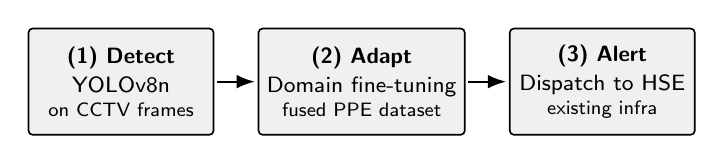
\begin{tikzpicture}[
  font=\footnotesize\sffamily,
  >=Latex,
  box/.style={
    draw,
    rounded corners=1.5pt,
    align=center,
    inner sep=3pt,
    minimum height=1.35cm,
    minimum width=2.35cm,
    line width=0.6pt
  },
  stage/.style={box, fill=gray!12},
  arrow/.style={->, thick, shorten >=1pt, shorten <=1pt}
]
  \node[stage] (s1) {%
    \textbf{(1) Detect}\\[1pt]
    YOLOv8n\\[-1pt]
    {\scriptsize on CCTV frames}};
  \node[stage, right=0.55cm of s1] (s2) {%
    \textbf{(2) Adapt}\\[1pt]
    Domain fine-tuning\\[-1pt]
    {\scriptsize fused PPE dataset}};
  \node[stage, right=0.55cm of s2] (s3) {%
    \textbf{(3) Alert}\\[1pt]
    Dispatch to HSE\\[-1pt]
    {\scriptsize existing infra}};
  \draw[arrow] (s1) -- (s2);
  \draw[arrow] (s2) -- (s3);
\end{tikzpicture}%
}
\caption{The three-stage pipeline: a pretrained YOLOv8 base (1) is fine-tuned on the composite domain-adapted dataset (2); flagged violations are dispatched over existing infrastructure (3).}
\label{fig:pipeline}
\end{figure}

\subsection{Dataset Construction}
\label{sec:methods-dataset}

No single public corpus covers the class mix of a chemical-processing site, so the training set fuses three public sources and one site-specific corpus under a single class map (Fig.~\ref{fig:datasets}). Roboflow PPE-Detection \cite{roboflowppe} contributes a helmet- and vest-centred detection benchmark typical of construction imagery. SH17 \cite{ahmad2024sh17} contributes 17 classes of PPE items and human body parts across varied industrial scenes. The Roboflow gas masks corpus \cite{roboflowgasmasks} (384 images) supplies instances of the gas-mask class that construction-skewed benchmarks barely cover.
All sources are merged into a unified ten-class map: Person, helmet, vest, gloves, boots, goggles, no\_helmet, no\_gloves, no\_goggle, and gas mask. The explicit negative classes (no\_helmet, no\_gloves, no\_goggle) let the detector localize the \emph{absence} of an item directly instead of inferring it from a missing detection.

\begin{figure}[t]
\centering
\resizebox{\columnwidth}{!}{%
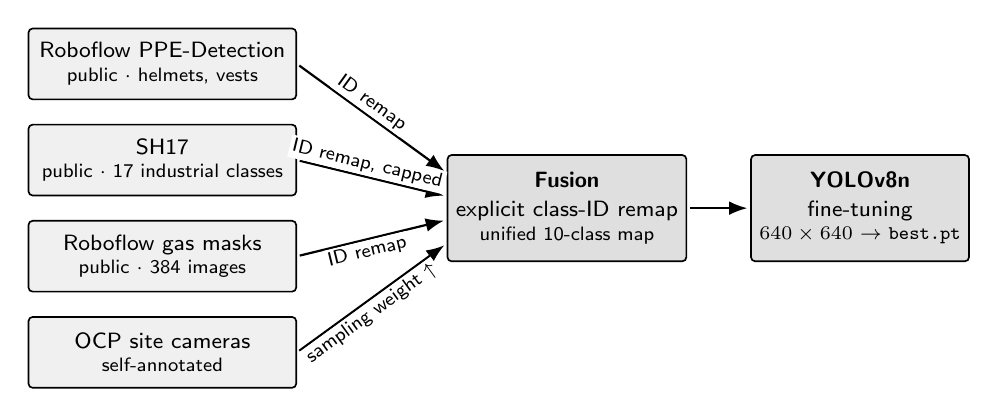
\begin{tikzpicture}[
  font=\footnotesize\sffamily,
  >=Latex,
  box/.style={
    draw,
    rounded corners=1.5pt,
    align=center,
    inner sep=3pt,
    minimum height=0.9cm,
    minimum width=3.4cm,
    line width=0.6pt
  },
  src/.style={box, fill=gray!12},
  proc/.style={box, fill=gray!25, minimum height=1.35cm, minimum width=2.7cm},
  arrow/.style={->, thick, shorten >=1pt, shorten <=1pt},
  note/.style={font=\scriptsize\sffamily, fill=white, inner sep=1pt}
]
  \node[src] (d1) {Roboflow PPE-Detection\\[-1pt]{\scriptsize public $\cdot$ helmets, vests}};
  \node[src, below=0.3cm of d1] (d2) {SH17\\[-1pt]{\scriptsize public $\cdot$ 17 industrial classes}};
  \node[src, below=0.3cm of d2] (d3) {Roboflow gas masks\\[-1pt]{\scriptsize public $\cdot$ 384 images}};
  \node[src, below=0.3cm of d3] (d4) {OCP site cameras\\[-1pt]{\scriptsize self-annotated}};

  \coordinate (mid) at ($(d2.east)!0.5!(d3.east)$);
  \node[proc, right=1.9cm of mid] (fuse) {\textbf{Fusion}\\[1pt]explicit class-ID remap\\[-1pt]{\scriptsize unified 10-class map}};
  \node[proc, right=0.8cm of fuse] (model) {\textbf{YOLOv8n}\\[1pt]fine-tuning\\[-1pt]{\scriptsize $640\times640$ $\rightarrow$ \texttt{best.pt}}};

  \draw[arrow] (d1.east) -- node[note, pos=0.45, above, sloped] {ID remap} ($(fuse.west)+(0,0.45)$);
  \draw[arrow] (d2.east) -- node[note, pos=0.45, above, sloped] {ID remap, capped} ($(fuse.west)+(0,0.15)$);
  \draw[arrow] (d3.east) -- node[note, pos=0.45, below, sloped] {ID remap} ($(fuse.west)+(0,-0.15)$);
  \draw[arrow] (d4.east) -- node[note, pos=0.45, below, sloped] {sampling weight $\uparrow$} ($(fuse.west)+(0,-0.45)$);
  \draw[arrow] (fuse) -- (model);
\end{tikzpicture}%
}
\caption{Dataset composition (stage 2 of Fig.~\ref{fig:pipeline}): four sources merged under a unified ten-class map with explicit label-ID remapping; SH17 is capped across all three splits (1,500 train, 300 validation, 300 test) to bound both fine-tuning and per-epoch validation cost, and only the OCP corpus receives a higher (\texttt{\(\times\)}3) sampling weight, since it is the deployment domain itself rather than a generic stand-in for one class. A held-out OCP portion forms the chemical-plant evaluation set (Section~\ref{sec:methods-comparison}).}
\label{fig:datasets}
\end{figure}

Fusing annotation sets is not file concatenation, and the remapping step deserves emphasis because its failure mode is silent. Each source's integer class IDs index that source's own ontology: SH17's IDs 0--16 reference its 17-class list, not the fused map. Under naive merging, in-range IDs are reinterpreted as the wrong class, and every image with an ID at or above the fused class count is silently discarded as corrupt; in a preliminary naive merge, this alone rejected roughly 43\% of training images. Our pipeline therefore remaps explicitly before merging: each SH17 class is mapped to its fused ID or deliberately excluded (body-part classes), the mapping is recorded, and all label files are rewritten before any image enters training.

SH17 also outnumbers the other three sources combined by roughly an order of magnitude (8{,}000 images against roughly 1{,}000: 308 from Roboflow PPE-Detection, 361 gas-mask images, 352 OCP images), and both remap cost and per-epoch training cost scale directly with pool size; because validation runs every epoch under the training framework's default policy, an uncapped validation split imposes this cost as well, not only an uncapped training split. Because well-represented classes (\emph{Person}, \emph{gloves}, \emph{vest}, \emph{no\_helmet}) saturate detector performance with a few hundred examples, we cap SH17's contribution to all three splits, drawn uniformly at random with a fixed seed: 1{,}500 training images, and 300 each for validation and test. This bounds fine-tuning and per-epoch validation cost on commodity compute (a single Colab GPU) without a material cost to accuracy on common classes, at the price of proportionally thinning classes already scarce within SH17 itself, and, for validation and test, of computing reported metrics on a fixed random subsample rather than the full corpus. Both trade-offs are returned to in Section~\ref{sec:discussion}.

The gas-mask class receives targeted treatment: respiratory protection is among the most safety-relevant items at chemical sites yet under-represented in construction-skewed public data, so the class is populated by the Roboflow gas masks corpus \cite{roboflowgasmasks}. Unlike the OCP corpus, gas-mask training images are not oversampled: the source is a generic public stand-in for a single class rather than the deployment domain itself, so duplicating it would add fine-tuning cost without the domain-relevance payoff that justifies OCP's higher sampling weight. Diversity within the class is instead addressed through the augmentation policy of Section~\ref{sec:methods-preprocessing} alone.

The fourth dataset component is a self-annotated corpus from OCP site cameras that captures conditions public data lacks: phosphate dust, harsh lighting transitions, and site-specific uniforms and equipment. This corpus has been collected and annotated against the fused class map using Roboflow's annotation tooling, and is included in the training mix. OCP samples receive a higher sampling weight than public samples, so each batch is biased toward deployment-realistic imagery while the public data preserves visual diversity. A held-out portion of the OCP corpus, disjoint from all training data, forms the chemical-plant evaluation set of the central comparison (Section~\ref{sec:methods-comparison}); publication of individual site frames remains subject to imagery clearance. The fused dataset is partitioned 70\%/15\%/15\% into training, validation, and test splits; the split is decided independently within each of the four source datasets (not stratified by class) before remapping and duplication, and a fixed seed makes it identical across runs.

\subsection{Preprocessing}
\label{sec:methods-preprocessing}

All images are resized to $640\times640$ pixels. The augmentation policy targets the visual failure modes of industrial CCTV. HSV jitter perturbs hue, saturation, and value to simulate the colour and contrast shifts produced by dust haze and glare. Horizontal flipping doubles pose variety. Random erasing imitates partial occlusion by equipment and other workers. Mosaic augmentation composites four training images to vary object scale and context, and is disabled for the final training epochs so that late optimization sees realistically composed frames.

\subsection{Model Training}
\label{sec:methods-training}

The detector is YOLOv8n \cite{ultralytics2023}, the nano variant of YOLOv8: 3.0M parameters, 8.1 GFLOPs at $640\times640$, and 6.3 MB of weights. The small footprint is deliberate: retrofit deployment means inference must run on commodity hardware alongside existing video infrastructure. Training runs on Google Colab for up to 50 epochs at $640\times640$ with batch size 16, stopping early if validation mAP does not improve over 20 consecutive epochs (patience 20); the reported run trained for the full 50 epochs without triggering the patience-based early stop. Optimizer selection is left to the framework's automatic policy, which configures an SGD-family optimizer with initial learning rate 0.01, momentum 0.937, and weight decay $5\times10^{-4}$; the first three epochs apply learning-rate warmup. The best checkpoint by validation fitness is exported as \texttt{best.pt} and used in all subsequent stages. Detection accuracy is reported in Section~\ref{sec:results}.

\subsection{Generic-vs-Adapted Comparison Protocol}
\label{sec:methods-comparison}

The central experiment asks whether generic benchmark training transfers to an operating chemical plant. The \emph{generic baseline} is the detector trained solely on the Roboflow PPE-Detection corpus \cite{roboflowppe}: 308 images over nine construction-oriented classes, with 58.1\% precision, 64.4\% recall, and 59.1\% mAP@50 on its own validation split. This is what a practitioner who deploys the public benchmark model obtains off the shelf. The \emph{industrial-adapted model} is the fused-dataset detector of Section~\ref{sec:methods-training}.

Both models are evaluated on two test sets neither saw during training: the held-out OCP site imagery of Section~\ref{sec:methods-dataset} (the headline comparison, since it is exactly the deployment domain) and an \emph{industrial proxy} set of held-out SH17 industrial scenes and gas-mask images \cite{roboflowgasmasks}, publishable without imagery clearance. Because the class inventories differ, metrics are computed over the classes common to both maps (person, helmet, vest, gloves, and their negative states) at identical resolution and confidence thresholds. The baseline also differs in training-set size, a confound discussed in Section~\ref{sec:discussion}; the comparison measures what the public benchmark model actually delivers on plant imagery, which is the deployment-relevant question.

\subsection{Alert and Deployment Architecture}
\label{sec:methods-alerts}

When the detector flags a violation above the operating confidence threshold, the dispatch stage pushes an alert (camera ID, violation class, detection confidence, and a timestamped clip) over the sites' existing network. Detector inference runs on commodity compute, so the pipeline requires no new capital hardware, and coverage is continuous: unlike a human operator, it has no attention span to exhaust.

\section{Results and Analysis}\label{sec:results}

% NOTE: All measured values in this section are \phX placeholders pending the
% training rerun (fixed SH17 remap + gas-mask class). Drop numbers in from the
% rerun log; do not reuse figures from the earlier fusion run.

The fused-dataset YOLOv8n detector reaches \phX\% precision, \phX\% recall, and \phX\% mAP@50 across all classes while processing a frame in \phX~ms on a Tesla T4-class GPU. That combination is the central finding of this section: accuracy sufficient for operational alerting, delivered at a speed and model footprint that fit the retrofit deployment model on existing CCTV infrastructure. Sections~\ref{sec:results-training} and~\ref{sec:results-perclass} report the detector's aggregate and per-class behavior, Section~\ref{sec:results-ocp} scopes the in-progress site-specific fine-tuning stage, Section~\ref{sec:results-cases} presents qualitative case studies of the LLM judge, Section~\ref{sec:results-errors} analyzes error structure, and Section~\ref{sec:results-runtime} quantifies runtime feasibility.

\subsection{Training Performance}\label{sec:results-training}

\begin{figure}[t]
\centering
% TODO: regenerate from rerun (fixed SH17 remap + gas-mask class); current file is from the superseded fusion run
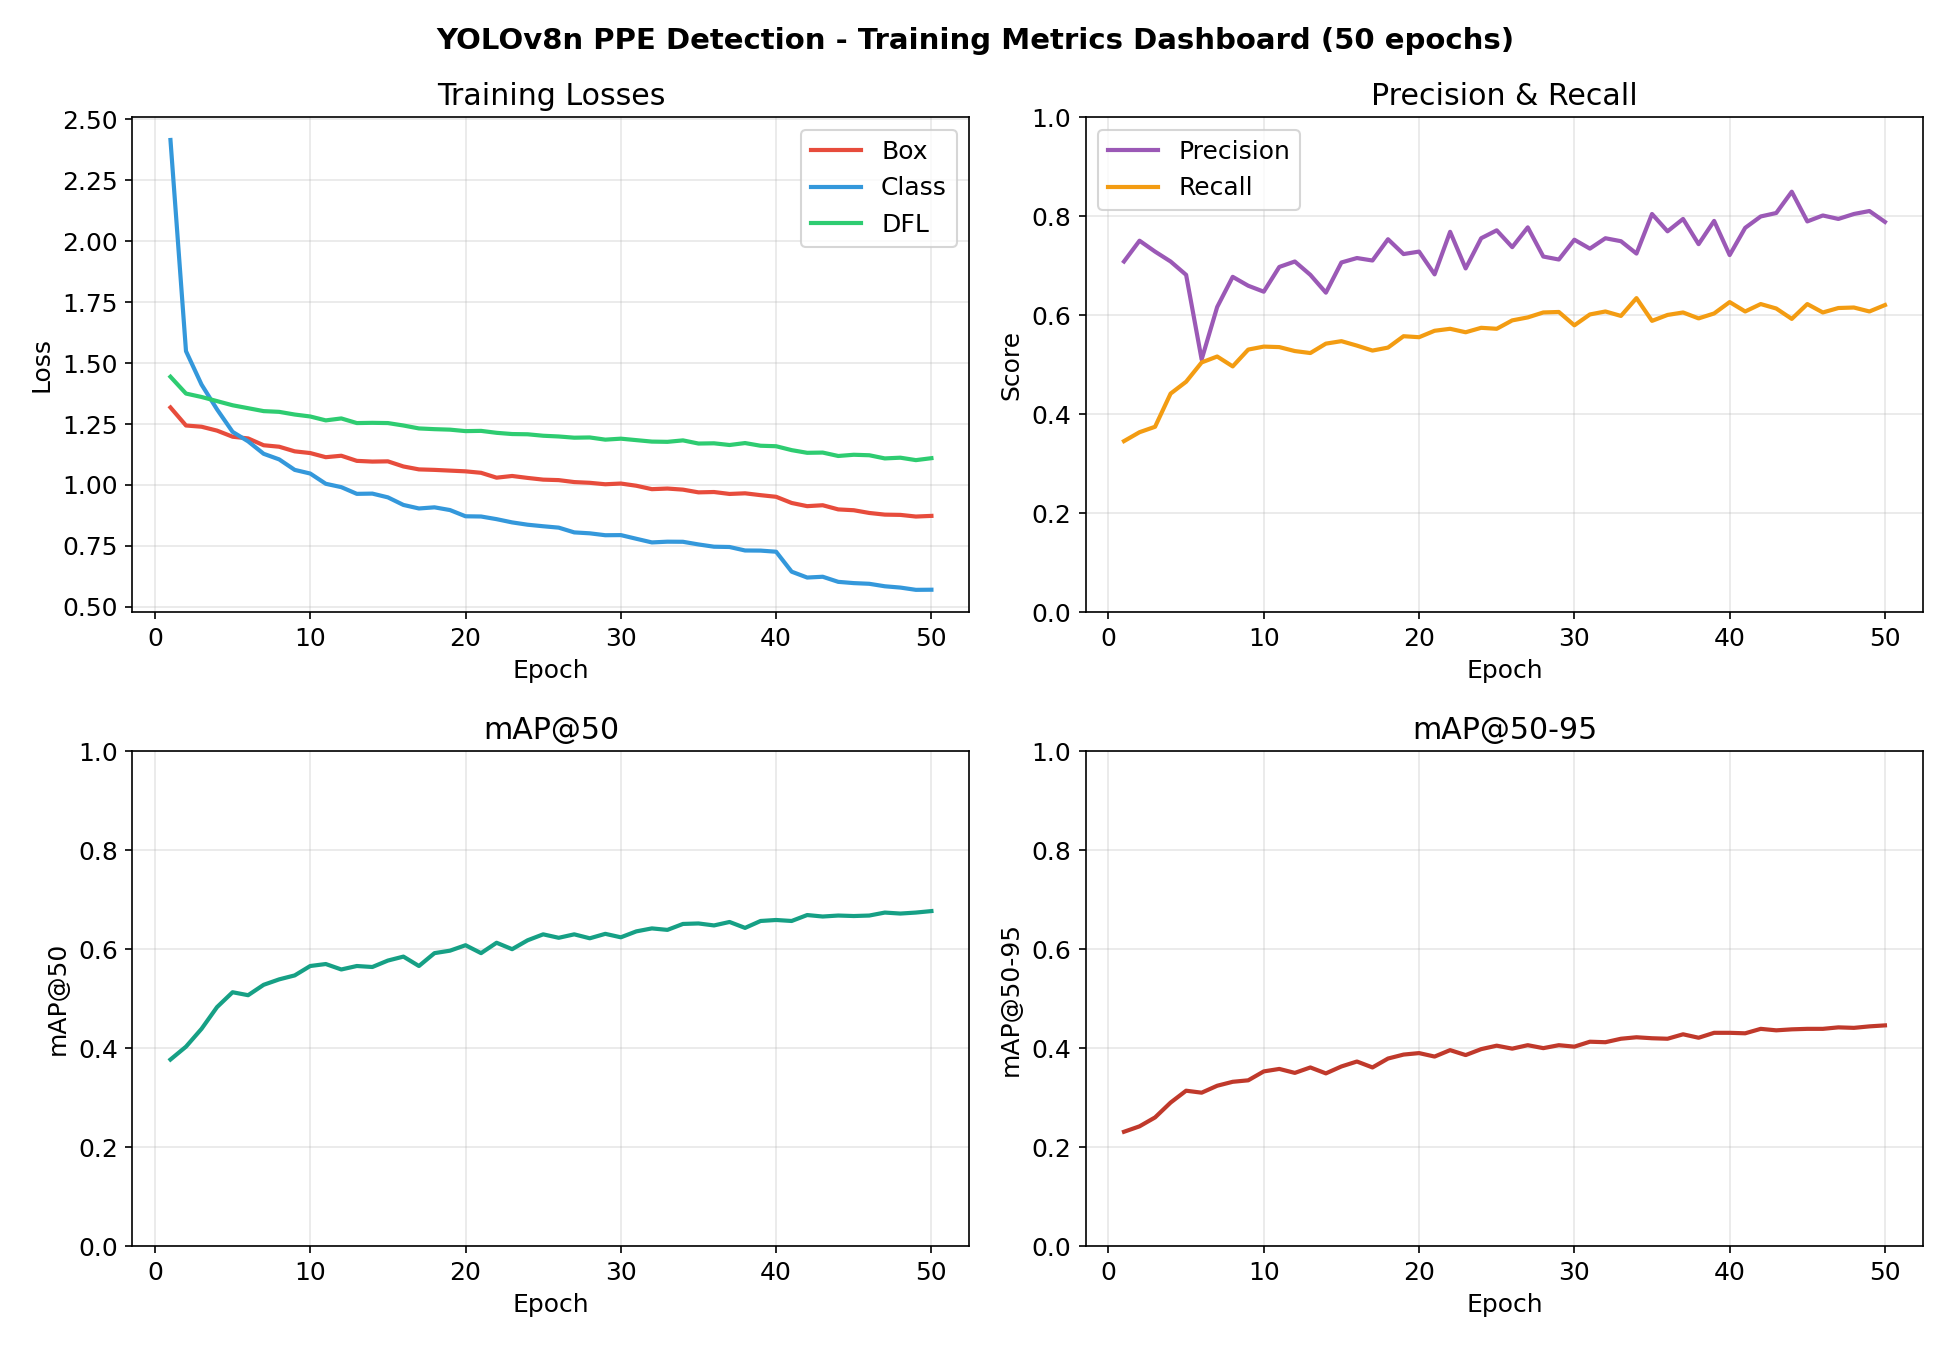
\includegraphics[width=\columnwidth]{figures/dashboard.png}
\caption{Training dashboard for the fused-dataset run: box, classification, and DFL loss curves (train and validation) with precision, recall, mAP@50, and mAP@50--95 per epoch.}
\label{fig:dashboard}
\end{figure}

Figure~\ref{fig:dashboard} summarizes the \phX-epoch training run at $640\times640$ input resolution with batch size 16. Box, classification, and distribution focal (DFL) losses decline from \phX, \phX, and \phX at the first epoch to \phX, \phX, and \phX at the final epoch, with validation losses tracking the training curves throughout. Precision and recall stabilize after approximately \phX epochs at \phX\% and \phX\% respectively. The final model attains \phX\% mAP@50 and \phX\% mAP@50--95 on the validation split. All headline values are taken from the best checkpoint (\texttt{best.pt}), selected on validation mAP@50--95. Unless noted otherwise, reported metrics use the \phX split of the fused dataset; the same split is used consistently across Table~\ref{tab:perclass} and the error analysis of Section~\ref{sec:results-errors}.
% TODO: decide val split vs. held-out test split for headline tables (structure.md open item); a held-out test set is the stronger claim.

\subsection{Detection Performance by Class}\label{sec:results-perclass}

Table~\ref{tab:perclass} breaks performance down by class. The fused dataset inherits markedly uneven per-class support from its source corpora \cite{roboflowppe, ahmad2024sh17}: person, helmet, and vest instances dominate, while negative-state classes (no\_helmet, no\_gloves, no\_goggle) and the gas-mask class introduced by this work's augmentation have far fewer validation instances. Rows for low-support classes should therefore be read alongside the support caveats in Section~\ref{sec:results-errors}, where the imbalance and its consequences are examined directly.

\begin{table}[t]
\caption{Per-class detection performance on the validation split. All values pending training rerun.}
\label{tab:perclass}
\centering
\begin{tabular}{lccc}
\toprule
Class & Precision (\%) & Recall (\%) & mAP@50 (\%) \\
\midrule
Person      & \phX & \phX & \phX \\
helmet      & \phX & \phX & \phX \\
no\_helmet  & \phX & \phX & \phX \\
vest        & \phX & \phX & \phX \\
gloves      & \phX & \phX & \phX \\
no\_gloves  & \phX & \phX & \phX \\
goggles     & \phX & \phX & \phX \\
no\_goggle  & \phX & \phX & \phX \\
boots       & \phX & \phX & \phX \\
gas mask    & \phX & \phX & \phX \\
\midrule
\textbf{All classes} & \phX & \phX & \phX \\
\bottomrule
\end{tabular}
\end{table}

\subsection{Effect of Site-Specific Fine-Tuning}\label{sec:results-ocp}

The OCP fine-tuning stage is in progress at the time of writing; no site-specific results are claimed here. The planned evaluation compares the generic fused-dataset model against the OCP-weighted model on an identical held-out set of site imagery, reporting per-class deltas and side-by-side qualitative detections under the dust, lighting, and uniform conditions that motivate the domain-adaptation stage. Figure~\ref{fig:ocp-compare} reserves the position for this comparison, pending completion of the fine-tuning run and clearance of site imagery for publication.

\begin{figure}[t]
\centering
\fbox{\parbox[c][4cm][c]{0.9\columnwidth}{\centering Placeholder: side-by-side detections,\\generic fused-dataset model vs.\ OCP-weighted model,\\on identical OCP site imagery.}}
\caption{Generic vs.\ OCP-weighted model on identical site imagery. TODO: pending OCP fine-tuning run and imagery clearance.}
\label{fig:ocp-compare}
\end{figure}

\subsection{LLM Judge Qualitative Case Studies}\label{sec:results-cases}

The judge stage is evaluated qualitatively. The protocol selects three to five real flagged detections from pilot footage and, for each, presents the detection crop, the verbatim \texttt{reason} field returned by the Qwen2.5-VL judge \cite{qwen25vl}, and the final verdict. The case set is chosen to include at least one false positive that the judge correctly rejects (for example, a glare or occlusion artifact of the kind that drives false-alarm load in manual CCTV monitoring \cite{donald2015}) and at least one genuine violation that the judge confirms, so that both failure-suppression and violation-preservation behavior are visible on real inputs. Table~\ref{tab:cases} holds the case scaffold.

We state explicitly: no quantitative false-positive-reduction figure is claimed for the judge stage anywhere in this paper. The case studies demonstrate the mechanism operating on real detections; they do not measure its aggregate effect. Quantitative benchmarking of the judge, over a labeled alert set with a confirm/reject confusion matrix, is future work (Section~\ref{sec:discussion}).

\begin{table*}[t]
\caption{LLM judge case studies: flagged detections with verbatim judge output. TODO: fill from pilot judge runs; include detection crops as an accompanying figure once imagery is cleared.}
\label{tab:cases}
\centering
\begin{tabular}{clcp{8.5cm}}
\toprule
Case & Flagged class & Judge verdict & Judge reason (verbatim) \\
\midrule
1 & TODO & TODO & TODO \\
2 & TODO & TODO & TODO \\
3 & TODO & TODO & TODO \\
4 & TODO & TODO & TODO \\
5 & TODO & TODO & TODO \\
\bottomrule
\end{tabular}
\end{table*}

\subsection{Error Analysis}\label{sec:results-errors}

Confusion concentrates among visually similar class pairs. The equipment/absence pairs (helmet vs.\ no\_helmet, goggles vs.\ no\_goggle) are separated by fine-grained head-region cues that degrade with distance and partial occlusion; \phX\% of no\_helmet errors fall into this pattern. Dark headwear and hoods account for a further \phX\% of helmet-related confusions, and gloves at long range are confused with bare hands in \phX\% of cases.

Class support shapes these figures. The helmet class holds \phX validation instances against \phX for no\_helmet, so the two rows in Table~\ref{tab:perclass} rest on very different evidence bases, and the same asymmetry applies to the other equipment/absence pairs. Boots, no\_goggle, and gas mask each fall below \phX validation instances; their per-class metrics carry wide uncertainty and are treated as indicative rather than conclusive. How much of the observed error structure stems from the multi-source fusion itself, from the nano-scale model capacity, or from support imbalance is a question the per-class numbers will settle once the rerun completes.
% TODO: after rerun, decide framing per [OPEN: results_posture] in chapter-plan.md (own weak classes openly vs. relax the caveats).

\subsection{Runtime and Deployment Feasibility}\label{sec:results-runtime}

Single-frame latency on a Tesla T4-class GPU is \phX~ms end to end: \phX~ms preprocessing, \phX~ms inference, and \phX~ms postprocessing at $640\times640$ resolution. At an analysis rate of \phX frames per second per camera, one GPU of this class sustains approximately \phX concurrent camera feeds, before any batching across streams.

The model itself is small: YOLOv8n comprises 3.0M parameters at 8.1 GFLOPs, with a 6.3~MB weight file \cite{ultralytics2023}, in line with edge-oriented PPE deployments \cite{edgeyolo2024}. Together these figures support the retrofit argument. A site's existing cameras keep their role as passive sensors; the entire detection workload for a multi-camera installation concentrates on a single commodity GPU server attached to the existing network, with no per-camera hardware and no replacement of the installed CCTV base. The judge stage adds latency only on the flagged-detection path, which is orders of magnitude sparser than the frame stream itself, so detector throughput governs feed capacity.

\section{Discussion}\label{sec:discussion}

The central lesson of this paper is that generic benchmark training does not transfer to an operating chemical plant: what a public construction-benchmark model delivers on plant imagery, and what an industrially adapted model delivers on the same frames, are different quantities, and the difference is the contribution. This section examines that design decision, adapting the detector to the environment it must watch, and closes with the limits of the present evaluation.

\subsection{Why Domain Adaptation Matters}

Public PPE corpora are dominated by construction imagery: near-frontal views, daylight, helmets and high-visibility vests \cite{roboflowppe,ppeyolo2024}. A phosphate-processing site violates each assumption: airborne dust lowers contrast, fixed CCTV cameras watch from high oblique angles at distances curated datasets rarely contain, and gas masks and goggles matter as much as helmets. The composite dataset answers these mismatches: fusion broadens pose, scale, and class coverage beyond any single source \cite{ahmad2024sh17}, the Roboflow gas masks corpus \cite{roboflowgasmasks} covers the class most specific to chemical processing, and weighted fine-tuning on the self-annotated OCP corpus closes the remaining site gap. The generic-versus-adapted comparison (Section~\ref{sec:results-comparison}) is the experiment this dataset was built for, and it is what separates the work from another YOLO variant: the evidence concerns what operating-plant imagery demands of training data, not the merits of a particular architecture.

\subsection{Limitations}

\begin{itemize}
  \item \textbf{Small and distant objects:} gloves and goggles occupy few pixels in wide CCTV views, and the nano-scale detector loses accuracy on them well before helmets or vests are affected.
  \item \textbf{Dust and weather:} heavy dust, rain, and low light plausibly push accuracy below the reported figures; robustness under these conditions has not been measured.
  \item \textbf{Gas-mask scarcity:} the class is deliberately not oversampled (Section~\ref{sec:methods-dataset}), so its effective training incidence is lower than OCP's or an earlier oversampled configuration would give it; augmentation adds visual variety but not additional distinct instances, and the class remains under-represented relative to its importance in chemical processing.
  \item \textbf{no\_goggle has no data:} despite occupying a slot in the fused ten-class map (Section~\ref{sec:methods-dataset}) and in the OCP annotation schema specifically, no\_goggle received zero labeled instances from any of the four sources in this run. It is not a thin class but an empty one. Its 0.0\% row in Table~\ref{tab:perclass} is consequently uninformative about detector capability; closing this gap requires deliberately annotating negative-goggle examples in a future OCP collection pass, not a training or evaluation change.
  \item \textbf{SH17 subsampling:} the caps on SH17's contribution (Section~\ref{sec:methods-dataset}: 1,500 training images, 300 each for validation and test) are a uniform random subsample, not stratified by class; classes already scarce within SH17 (e.g., boots, helmet) are thinned in the same proportion as abundant ones. Because the caps now also apply to validation and test, reported metrics are computed on a fixed 300-image random subsample of SH17's held-out splits rather than the full source, which was not previously the case; this trades some evaluation coverage for a wall-clock training budget that fits available compute. A class-aware cap that preserves rare-class density, and a check of whether the smaller SH17 eval subsample shifts reported metrics, are candidate refinements.
  \item \textbf{Comparison confounds:} the generic baseline is trained on far less data than the fused corpus, so the comparison measures what deploying the public benchmark model actually yields on plant imagery, not the isolated effect of domain coverage; a size-matched control is future work.
  \item \textbf{Camera placement:} the system inherits the blind spots of the existing CCTV layout; better detection cannot compensate for uncovered areas.
  \item \textbf{OCP imagery release:} the self-annotated site corpus and fine-tuning stage are complete, but public release of OCP frames remains restricted overall; Figure~\ref{fig:ocp-compare} shows one cleared frame as a qualitative illustration, not a representative sample, and the held-out OCP evaluation set itself remains unpublished.
\end{itemize}

\section{Conclusion and Future Work}\label{sec:conclusion}

Industrial PPE monitoring fails not for lack of cameras but for lack of sustained attention. We presented a pipeline that retrofits detection and verification onto the CCTV infrastructure a site already owns: a YOLOv8 detector fine-tuned on a composite, domain-adapted dataset, and a vision-language-model judge that reviews each flagged event before it becomes an alert. The dataset is the core contribution: fusion of the public Roboflow PPE-Detection corpus with SH17 \cite{roboflowppe,ahmad2024sh17}, augmentation of the scarce gas-mask class, and weighted sampling that favors self-annotated OCP imagery from the deployment domain. On the fused data the detector attains \phX{} mAP@50 and \phX{} recall at \phX{}\,ms per frame, accuracy and speed compatible with multi-camera deployment on commodity hardware.

Future work proceeds in order of what the argument needs most. First, quantitative benchmarking of the judge on a labeled alert set, reporting its confirm/reject confusion matrix against human ground truth. Second, expansion of the OCP dataset across sites and seasons, completing the fine-tuning stage this paper describes as in progress. Third, temporal tracking and person re-identification, so that compliance is assessed per worker over time rather than per frame. Fourth, edge deployment to cut per-camera latency and network load \cite{edgeyolo2024}. Fifth, integration with access-control and IoT systems so that verified violations can gate entry to hazardous zones. The ordering is deliberate: until the judge is measured, the pipeline's central claim rests on design rationale, and measuring it costs less than any extension that follows.

\section*{Acknowledgment}
% TODO: confirm wording with partners
The authors thank OCP Group for site access and collaboration on the deployment study, and EMSI Marrakech for institutional support.

\section*{Data Availability}
The public datasets used in this work are available from their original sources \cite{roboflowppe,ahmad2024sh17}. Imagery collected at OCP sites is proprietary and cannot be made publicly available.


\bibliographystyle{IEEEtran}
\bibliography{references}

\end{document}
